\documentclass[oneside,12pt]{article}          % ----- article

\input{../../Latex/inputs/loading_packages.tex}			% ----- Packages utiles
\input{../../Latex/inputs/preambule_general.tex}         	% ----- Préambule feuilles de TD
\input{../../Latex/inputs/mymacros.tex}                 % ----- Macros mathématiques
\input{../../Latex/inputs/mise_en_page.tex} 		   	% ----- Macros de mise en page

\fancyhead[R]{Accompagnement de stage}
\fancyhead[C]{Maîtriser les TICE}
\fancyhf[CF]{\footnotesize{Master M2E - S3}}


\titlespacing{\section}{0pt}{2mm}{0pt}
\titlespacing{\subsection}{0pt}{5mm}{1mm}


%%%%%%%%%%%%%%%%%%%%%%%%%%%%%%%%%%%%%%%%%%%%%%%%%%%%%%%%%%%%%%%%%%%%%%%%%%%%%%%%%%%%%%%%%%%%%%%%%%%%%%%%%%%%%
%%%%%%%%%%%%%%%%%%%%%%%%%%%%%%%%%%%%%%%%%%%%%%%%%%%%%%%%%%%%%%%%%%%%%%%%%%%%%%%%%%%%%%%%%%%%%%%%%%%%%%%%%%%%%
%%%%%%%%%%%%%%%%%%%%%%%%%%%%%%%%%%%%%%%%%%%%%%%%%%%%%%%%%%%%%%%%%%%%%%%%%%%%%%%%%%%%%%%%%%%%%%%%%%%%%%%%%%%%%


\begin{document}

\section{Théorème de Varignon}

\begin{theoreme}{Théorème de Varignon}

	\begin{minipage}{0.6\textwidth}
		Si ABCD est un quadrilatère quelconque et I, J, K, L les milieux de ses côtés, alors IJKL est un parallélogramme, appelé parallélogramme de Varignon du quadrilatère.
	\end{minipage}
	\begin{minipage}{0.3\textwidth}
		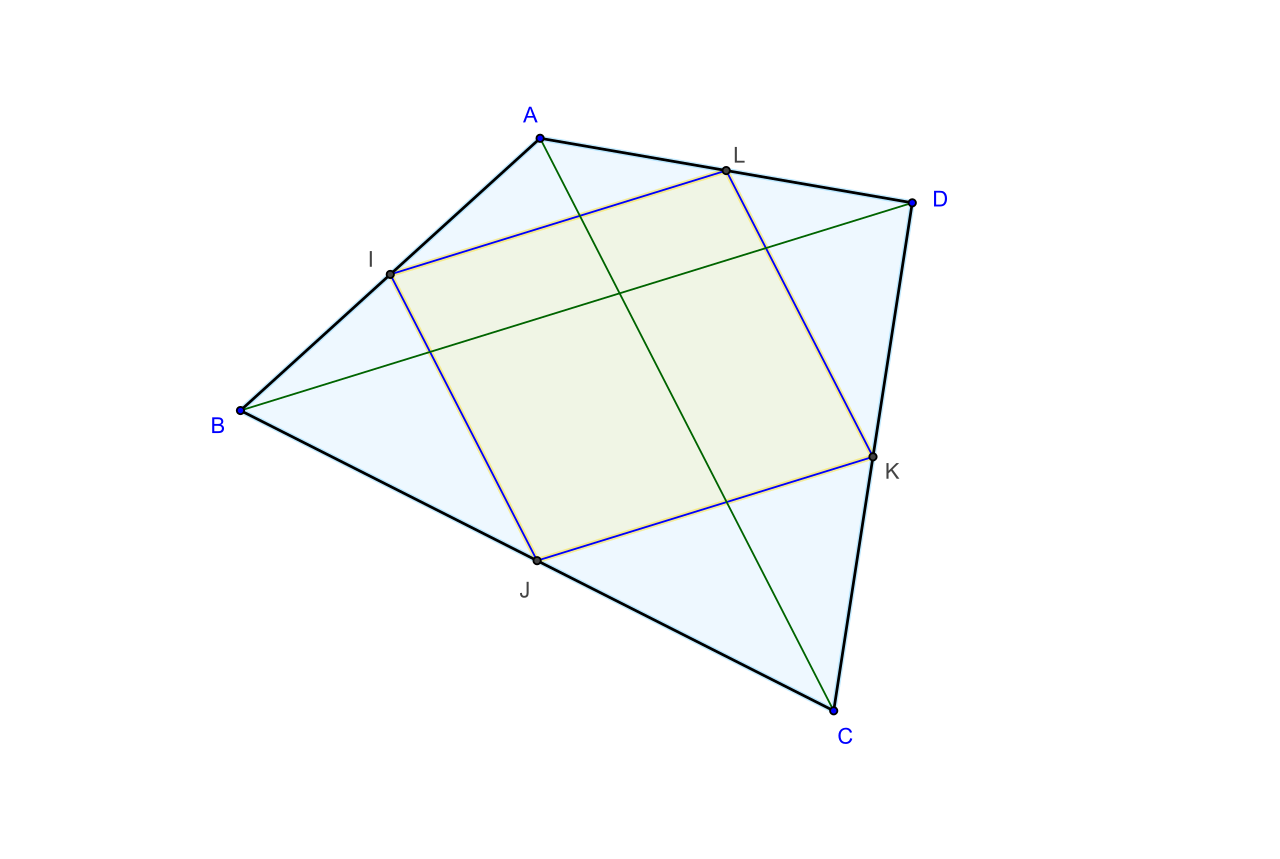
\includegraphics[scale=0.2]{varignon.png}
	\end{minipage}
\end{theoreme}


\section{Preuve de l'aire du parallélogramme de Varignon}

\begin{propriete}{Aire du parallélogramme de Varignon}
	L'aire du parallélogramme de Varignon est égale à la moitié de l'aire du quadrilatère dans lequel il s'inscrit.
\end{propriete}


On considère un quadrilatère quelconque $ABCD$ et on note $M$ , $F$ , $G$ et $H$ les milieux respectifs des segments $[AB]$ , $[BC]$ , $[CD]$ et $[AD]$

On appelle $J$ l'intersection de $(MH)$ et $(AC)$

On appelle $K$ l'intersection de $(FG)$ et $(AC)$

On note $O$ le point d'intersection des droites $(MF)$ et $(BD)$



\subsection{Découper \& recoller la figure par symétrie centrale}

On considère le point $P$ image de $S_1$ la symétrie centrale de $J$ par rapport à $M$ \\
On peut constater que le triangle $MPB$ est alors l'image du triangle $AJM$ par la même symétrie.

On considère le point $N$ image de $S_2$ la symétrie centrale de $K$ par rapport à $F$ \\
On peut constater que le triangle $FBN$ est alors l'image du triangle $KFC$ par la même symétrie.



\subsection{Démontrer / Justifier que les points P , B et N sont alignés}

\begin{propriete}{Image par une symétrie}
	L'image d'une droite par une symétrie centrale $S$ est une droite parallèle à son antécédent.
\end{propriete}

$(PB)$ est l'image par $S_1$ de $(AJ)$ , donc $(PB) // (AJ)$ \\
$(BN)$ est l'image par $S_2$ de $(KC)$ , donc $(BN) // (KC)$

Or les droites $(AJ)$ et $(KC)$ sont confondues, donc $(PB)$ est parallèle à $(BN)$ par transitivité du parallélisme.

Le point $B$ appartenant à ces deux droites, on peut conclure qu'elles sont confondues, autrement dit les points $P$ , $B$ et $N$ sont alignés.



\subsection{On justifie la nature de $MFKJ$}

\begin{theoreme}{Droite des milieux}
	Si un segment joint les milieux de deux côtés d’un triangle, alors il est parallèle au troisième côté, et sa longueur est égale à la moitié de celle de ce troisième côté
\end{theoreme}

Dans le triangle $ABC$, le segment $[MF]$ joint les milieux des segments $[AB]$ et $[BC]$ , donc d'après le théorème de la droite des milieux, les droites $(MF)$ et $(AC)$ sont parallèles.

A fortiori les droites $(MF)$ et $(JF)$ sont parallèles.

En appliquant le même raisonnement dans le triangle $ABD$, on démontre que les droites $(HM)$ et $(BD)$ sont parallèles.

De même dans le triangle $BCD$, on démontre que les droites $(FG)$ et $(BD)$ sont parallèles.

Par transitivité du parallélisme, les droites $(HM)$ et $(GF)$ sont parallèles, on peut donc conclure que le quadrilatère $MFKJ$ est un parallélogramme.



\subsection{On justifie que $(JP) // (KN)$}

Comme $S_1$ est une symétrie de centre $M$ et $P = S_1(J)$ , on peut conclure que  $M$ est le milieu de $[JP]$ \\
Donc $J$ , $M$ et $P$ sont alignés.

Comme $S_2$ est une symétrie de centre $F$ et $N = S_2(K)$ , on peut conclure que  $F$ est le milieu de $[KN]$\\
Donc $K$ , $F$ et $N$ sont alignés.

Donc les droites $(JP)$ et $(KN)$ sont parallèles.



\subsection{On conclut quant à la nature de $JKNP$}
On a montré que $(JP) // (KN)$ et $(PN) // (JK)$ donc le quadrilatère $JKNP$ est un parallélogramme.



\subsection{On remarque que $PNKF$ se découpe en deux parallélogrammes de même aire}

Comme $PNKF$ est un parallélogramme et que $M$ et $F$ sont les milieux respectifs des segments $[JP]$ et $[KN]$, on peut conclure que les deux quadrilatères $JMFK$ et $MPNF$ sont deux parallélogrammes superposables, donc ils sont de même aire.


\subsection{On conclut quant à l'aire du parallélogramme $MFGH$}
Par recollage, on vient de montrer que $\Acal_{AMJ} + \Acal_{MBF} + \Acal_{CKF} = \Acal_{MFKF}$ \\
Donc $\Acal_{ABC} = 2 \times \Acal_{MJKF}$

Par symétrie du raisonnement on peut également démontrer que $\Acal_{ADC} = 2 \times \Acal_{JKGH}$ 

Par additivité de l'aire on obtient $\Acal_{ABCD} = 2 \times \Acal_{MFGH}$



\section{Figure explicative}

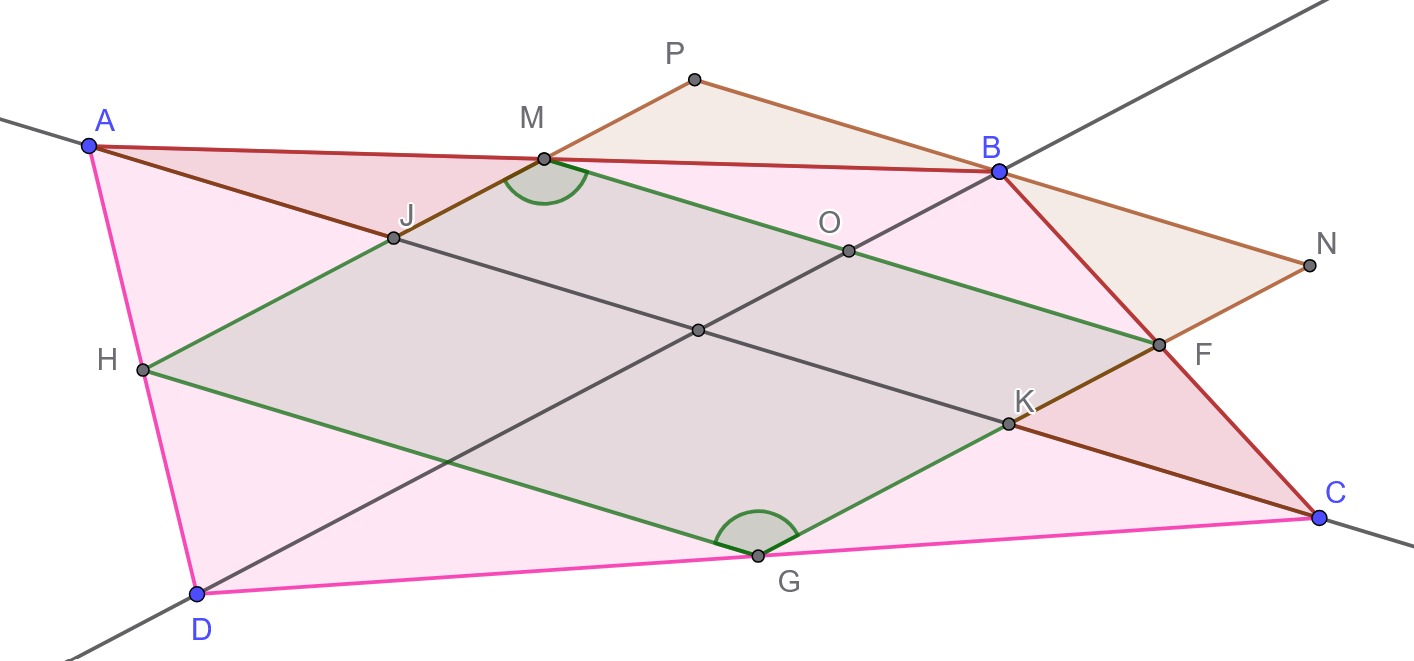
\includegraphics[scale=0.4]{symetries.jpeg}





\end{document}
